\documentclass[11pt, english]{scrartcl}

\usepackage[utf8]{inputenc}
\font\myfont=cmr11 at 60pt
\title{Test report\\~\\~\\~\\{\myfont Outlr\textcolor[HTML]{925FF0}{.}}}
\subtitle{A web application for analyzing subspace-outliers on high dimensional datasets}
\author{Bennet Alexander Hörmann, Salomo Hummel,\\
Simeon Hendrik Schrape, Erik Bowen Wu, Udo Ian Zucker}

\usepackage{tabularx}
\usepackage{blindtext}
\usepackage{hyperref}
\usepackage[T1]{fontenc}
\usepackage[ddmmyyyy]{datetime} % must be after babel
\renewcommand{\dateseparator}{.}
\usepackage[margin=1.6in]{geometry} % Page margins
\usepackage{amsmath} % for $\text{}$
\usepackage[nameinlink]{cleveref}
\usepackage[section]{placeins}
\usepackage{xcolor}
\usepackage{svg}
\usepackage{graphicx}
\usepackage[acronyms, toc]{glossaries}
\usepackage[toc, page]{appendix}
\usepackage{parskip} % Adds vertical space to paragraphs instead of indentation
\usepackage{outlr} % our own package

\hypersetup{
	pdftitle={Test report},
	colorlinks=true,
        allcolors = [HTML]{045c5c}
}

% Glossary setup
\makeglossaries
\loadglsentries{glossaries}

\begin{document}

\maketitle\pagebreak

\tableofcontents\pagebreak

\section{Fixed bugs}

\bugFix{The accuracy calculation after running an \gls{ODM} is flawed. }{
    After viewing the results of an \Gls{experiment} the accuracy is always displayed incorrectly as 0.
}{
    When converting the ground truth \gls{CSV} to a \gls{numpy} array, the header was included, even though the ground truth does not have one. This led to a data loss of one row. Then the accuracy calculation was done using our own method, which compares two \gls{numpy} arrays in a single statement. However, when comparing two arrays of different size, it will always return 0, thus leading to this bug.
}{
    Now, we fixed the conversion and use the accuracy method from scikit-learn to ensure accurate results.
}

\bugFix{The user is not redirected from routes requiring authentication when authentication "suddenly" is not valid anymore, even after a single page reload}{
    The token expire event is not handled, when a page requiring authentication is already loaded. This way, the user is seemingly able to communicate with the backend although not being logged in, that is the user seeminly has a valid access token. Since no request is responded to with useful information the user might reload the page, which however, also does not directly redirect to the login page. This way, the user is in a state where nothing seems to work as the user is not redirected to login page nor is able to send requests to the backend.
}{
    The token expire event is not handled correctly as the \code{isAuthenticated} state is not set when the token expires. Even if this state was properly set according to token validity, no action would take place since the authentication state has to be listened to.
}{
    Now, the user is redirected when the user triggers a component sending a http request to the backend. Furthermore, a single page reload now redirects to the login page when a route requiring authentication is trying to be accessed. This was handling the token expiration event correctly on frontend side by setting the Vuex state according to the token's validity when http requests are sent as well as listening to the Vuex state change (similarly to observer pattern) by subscribing to the state change.
}

\bugFix{Running \glspl*{experiment} can fail}{
    Running an \gls*{experiment} sometimes raises an exception from \gls{SQLAlchemy}.
}{
    Every API request uses the same \gls*{SQLAlchemy} session. The objects that are created and modified during the execution are still in the session while the experiment is running. (Objects with relationships to objects that are already in the session will automatically be added to the session.) When the session is automatically flushed or when it is flushed by another API request while the experiment is still running, \gls*{SQLAlchemy} needs to work with these objects. But they can be in a state that is not accepted by the database. For example, the \code{execution\_time} of \code{ExperimentResult} must not be \code{None}, but can only be defined after the execution has been completed. In this case, \gls*{SQLAlchemy} raises an exception.
}{
    Now each API Request has its own session as it is intended by the \gls*{SQLAlchemy} documentation.
    Additionally, the API request that starts the execution now closes the session before starting the execution and uses a second session to write the changes back to the database once the execution has finished.
}

\bugFix[wrong-odm-exceptions]{Exceptions from \glspl{ODM} too unspecific}{
    Exceptions raised by \glspl{ODM} should be instances of \code{ODMFailureError}. Instead, they are instances of more general exception classes.
}{
    Exceptions from \glspl{ODM} are not wrapped in the \code{ODMFailureError} exception class.
}{
    Now, exception handling is added to the \code{PyODM} class to raise \code{UnknownODMError}s and \code{ODMFailureError}s.
}


\bugFix{Exceptions from \glspl{ODM} not caught}{
    Exceptions raised by \gls{PyOD} \glspl{ODM} are not caught when using the \code{ExecutorODMScheduler} with a \code{ProcessPoolExecutor}. This causes the execution to crash instead of finish with an error. It can also lead to a broken process pool with the following error message: \emph{BrokenProcessPool: A process in the process pool was terminated abruptly while the future was running or pending.}
}{
    The exceptions that are raised by \code{PyODM.run\_odm} are constructed using keyword arguments. When constructing them by passing the same arguments without a keyword, the bug does not occur. It is unclear why this happens.
}{
    The given exceptions are now constructed using positional arguments.
}


\bugFix{kwargs}{
    'kwargs' parameters are recognized as mandatory but are optional.
}{
    They do not have a default value.
}{
    Set parameters named 'kwargs' to optional.
}

\section{Unfixed bugs}

% Write all bugs that we intend to fix in the fixed bugs section. If we don't fix it we can move it here in the end

\bugWithoutFix{Executor shuts down\notReproducible}{
    When scheduling an experiment sometimes one of the following exceptions is raised
    \begin{itemize}
        \item \emph{RuntimeError: cannot schedule new futures after interpreter shutdown}
        \item \emph{RuntimeError: cannot schedule new futures after shutdown}
    \end{itemize}
}{
    Unknown. The bug occurs rarely and cannot be reproduced reliably. It could be caused by modifying a python file while the server is running.
}

\bugWithoutFix{Supervised methods are displayed but not runnable}{
    Supervised methods are not supported but displayed on the create Page.
}{
    When scraping the PyOD module the methods are not checked on whether they are supervised or unsupervised.
}

\section{Improvements}

\improvement{Remove Dataset Class}{
    The \code{Dataset} class bundles the dataset name and the \gls{pandas} \code{DataFrame}. But since the dataset name is stored in the database there must be a single attribute for it. The \code{Dataset.name} is therefore never used.
}{
    Instead of a \code{Dataset} class \gls{pandas} \code{DataFrame}s are used directly.
}

\improvement{Improve Execution}{
    The experiment execution is built around the \gls{asyncio} library.
}{
    The experiment execution is now built around the \gls{concurrent-futures} library. This library is better suited for CPU-bound tasks while \gls{asyncio} is better suited for IO-bound tasks.
    However, the benefits of \gls{asyncio} are still used, since the two libraries are compatible.
    In particular, experiments are now executed as coroutines in an \gls{asyncio} event loop that runs on a single background thread. There, the subspace logic evaluation, metrics calculations, and the waiting for the individual \glspl{subspace} is done. The individual \glspl{subspace} however, are run in a \gls{concurrent-futures} \code{ProcessPoolExecutor}, which holds a pool of processes to distribute individual \gls{ODM} calls.
}

\improvement{Better \Gls*{subspace-logic} Parser}{
    Multiple operators are possible, but they can be applied only right associatively. The simple case of \code{([0] or [1]) and ([2] or [3])} is not possible.
    Additionally, many incorrect inputs are accepted.
}{
    Now, \gls{subspace-logic} can be nested using parenthesis. Many cases of incorrect inputs are caught and not parsed.
}

\improvement{Dashboard Table Metadata}{
    Table sorting was accomplished by comparing the string values of each cell.}
{
    Each cell now contains a tuple with both metadata and string representation. This allows for more accurate sorting, as the rows can be sorted based on the metadata of each cell rather than simply comparing string values.
}

\improvement{Dashboard Table Sorting Options}{
    Table sorting was reliant on the header strings to indicate which cell the table should be sorted by.
}{   
    Each table header now contains a tuple consisting of a Sort Enum entry and the header string. This Enum makes the sorting selection process easier and more efficient.
}

\improvement{Dashboard Table Date Shown}{
    The date on the dashboard table was previously displayed in a standard date format.
}{
    Now, when an experiment is created less than a week ago, the time is shown as [time] ago.
}

\improvement{Show \Gls*{subspace-logic} on \Gls*{experiment} Result Page}{
    \Gls{subspace-logic} is never displayed after an \gls{experiment} is created.
}{
    The \gls{subspace-logic} of an \gls{experiment} is displayed on the \gls*{experiment} result page.
}

\improvement{Subspace Logic Indicator}{
    Incorrect subspace logic was indicated by an unusable button.
}{
    Now, incorrect subspace logic is directly indicated on the text area field with a red border. The button is still unusable with incorrect subspace logic.
}

\improvement{Enhanced Password Storage Security}{
    Password were stored in the database after being hashed with the SHA-256 hashing algorithm.
}{
    Passwords now are hashed using bcrypt, which is specifically designed for password hashing. Bcrypt incorporates a cost parameter that makes the hashing process deliberately slower. This means that each password hash computation takes a longer time to complete, making it much more difficult for attackers to perform brute force attacks. It also includes salting as part of its hashing process, further increasing the security of the password hash.
}

\improvement{Minor Improvement to User Experience when Registering}{
    The green color used to mark valid input was quite bright.
}{
     The color to mark valid input was changed to a more subtle green. 
}

\improvement{AUC and ROC Curve}{
    The AUC and ROC Curve was neither stored in the database nor displayed to the user.
}{
    The AUC and ROC Curve are stored in the database. They get displayed to the user on the experiment result page.
}

\section{Unit tests}

We have utilized the unittest package for Python to ensure good quality in our backend. By creating a comprehensive suite of unit tests, we are able to systematically test individual units of code in isolation, ensuring that each function and method works as expected. 

To ensure that our unit tests cover as much of the codebase as possible, we have also utilized the coverage package for Python. This package allows us to measure how much our unit tests exercise the codebase. By analyzing the results of code coverage reports, we can identify areas of the codebase that are not being tested and prioritize efforts to improve test coverage.

On the frontend side, we utilized the Jest testing framework as our unit test package for TypeScript. Jest is a popular testing framework used for testing Vue applications and is highly regarded for its ease of use and powerful features. Since Jest already includes coverage we didn't need another framework in the frontend.

Overall we achieved $\geq 90 \%$ code coverage on both front and backend as documented in the following pictures. 

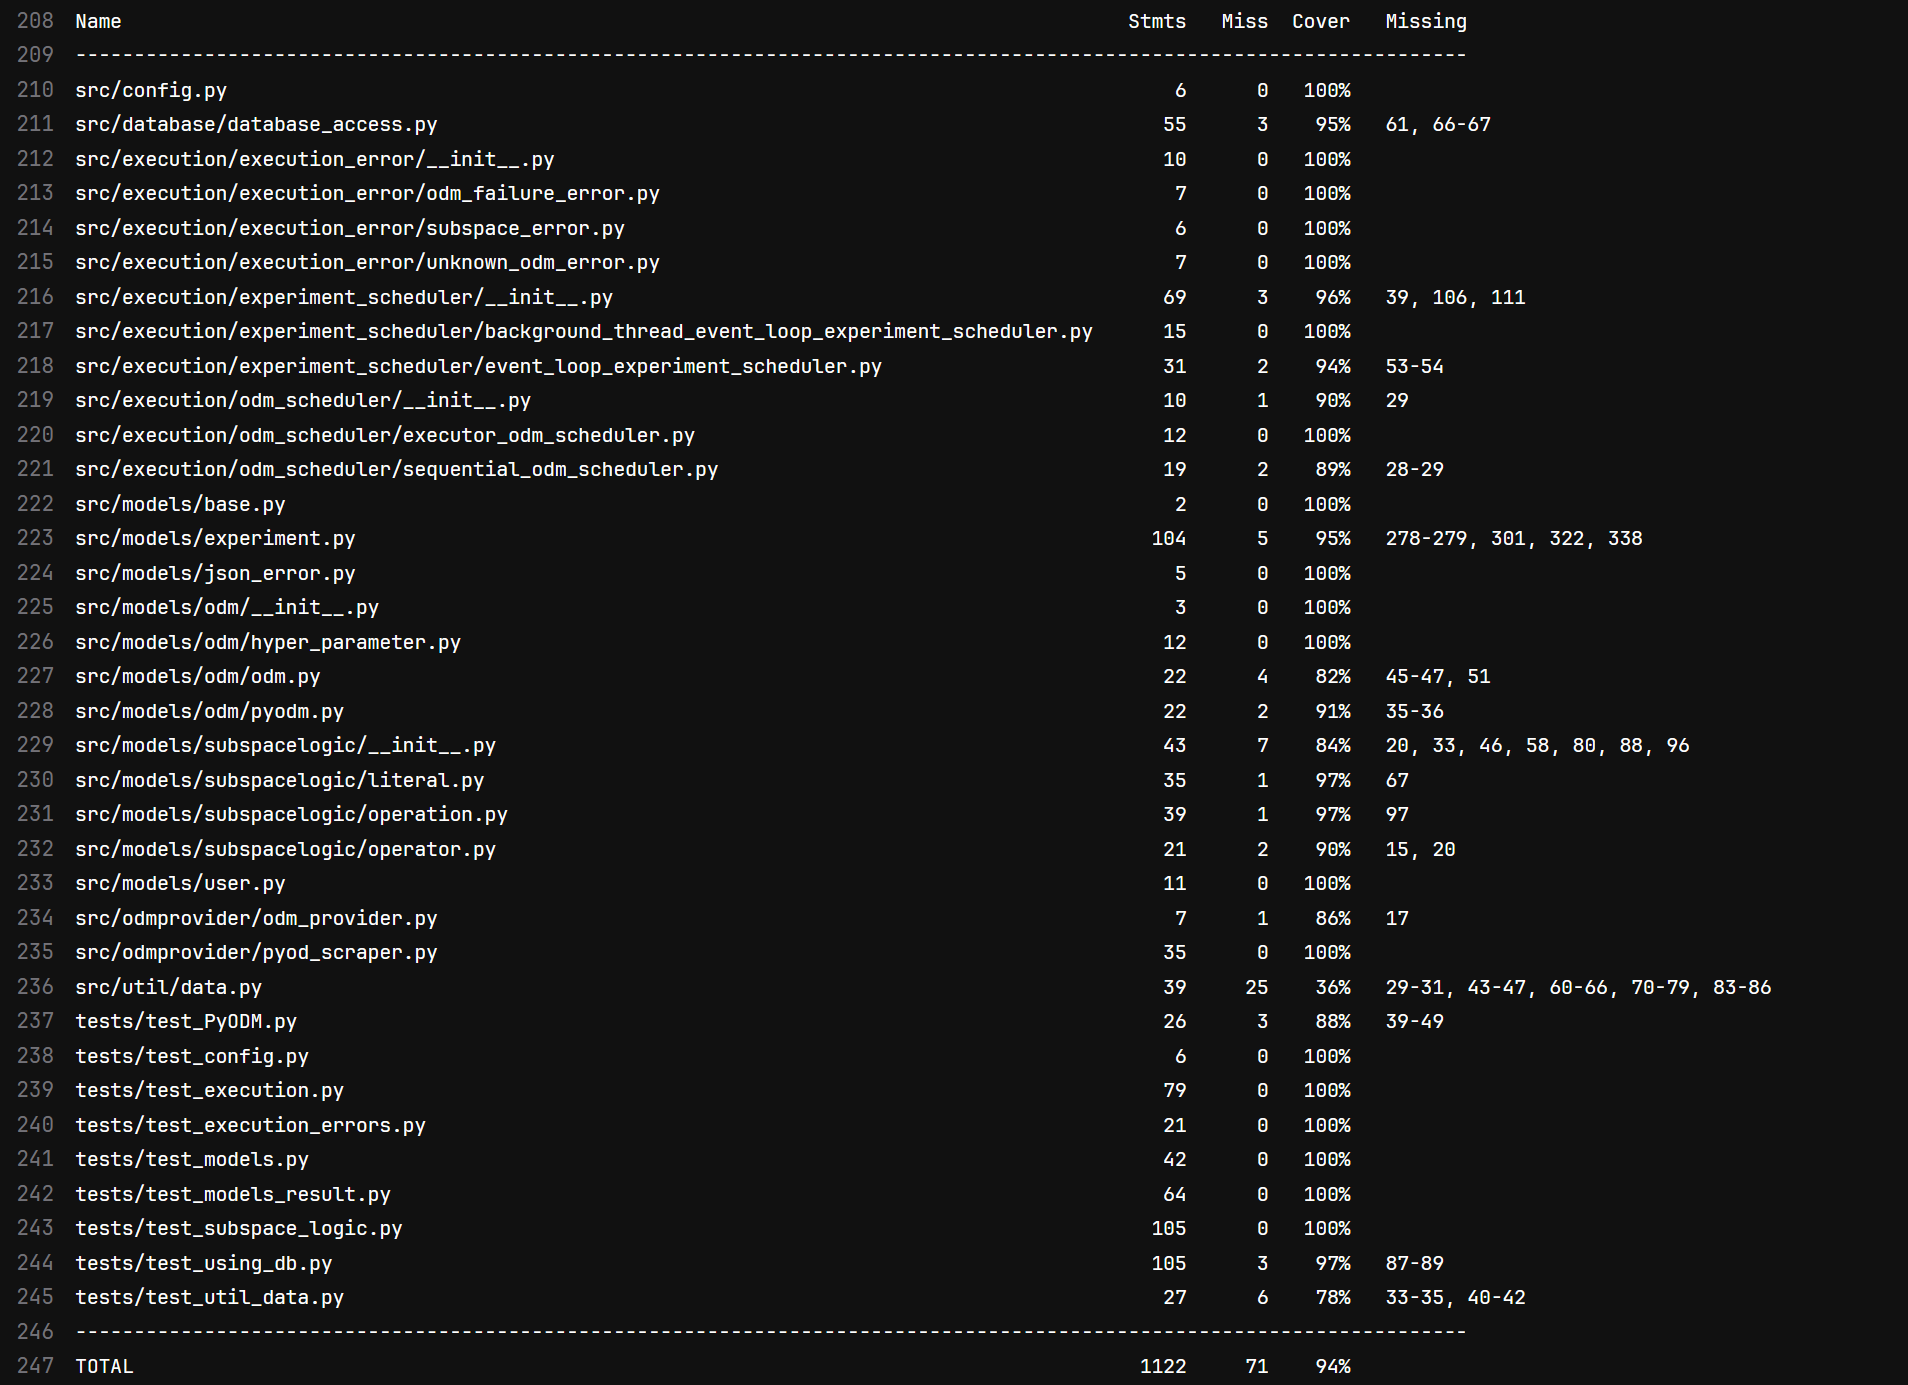
\includegraphics[width=1\textwidth]{images/backend.png}
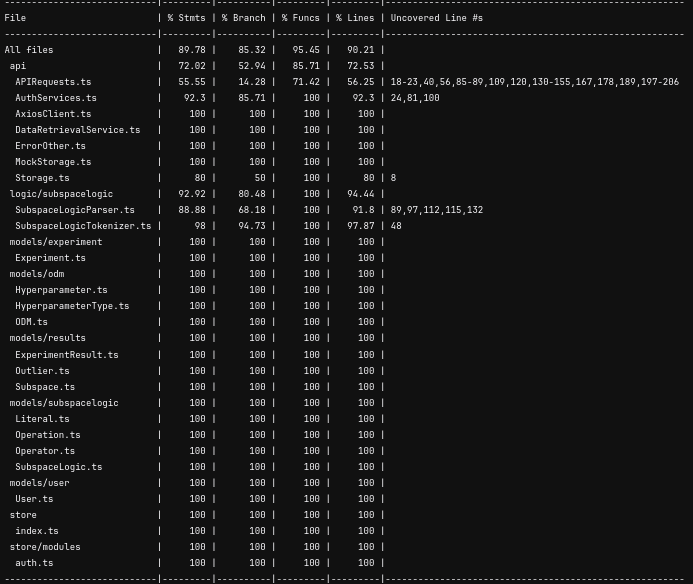
\includegraphics[width=1\textwidth]{images/frontend.png}

% \section{Integration Tests}
\todo{Did we do any API tests?}

% \include{sections/system-tests}
\section{Code Quality}

Static code analysis is an effective method for detecting defects and vulnerabilities in software code. It involves the use of automated tools to analyze code without actually executing it. One of the most common types of static analysis is linting, which checks code for syntax errors, style violations, and other potential issues. Our Code now has 0 lint issues.



\section{CI/CD Pipeline}
We maintained and extended our Gitlab CI/CD Pipeline to a three-step process. The first one builds the web application and prepares our PostgreSQL database. In the second step, we execute our backend and frontend unit tests. And lastly, we check for code smells and style with our linter.

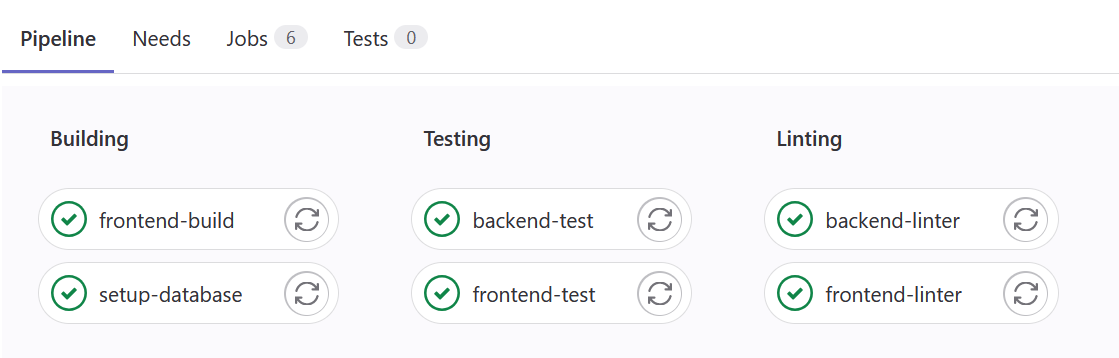
\includegraphics[width=1\textwidth]{images/pipeline.png}


This three-step process in our Gitlab CI/CD pipeline has been extremely beneficial for our testing phase.

Firstly, by building the web application and preparing the PostgreSQL database in the initial step, we ensure that all necessary dependencies are installed and the environment is properly set up. This helps us avoid any errors or issues that may arise from missing dependencies or configuration problems.

Secondly, executing backend and frontend unit tests in the second step ensures that all changes made to the codebase do not break existing functionality. The unit tests act as a safety net that helps us catch any issues or bugs before they make it to the production environment. By running the tests in an automated way through the CI/CD pipeline, we can ensure that the tests are always run consistently, and we can easily detect issues as soon as they arise.

Finally, the third step in our pipeline checks for code smells and style with our linter. This helps us maintain a high level of code quality and consistency throughout the project. By catching potential issues with code style or best practices early on, we can avoid issues and ensure that the code is easy to maintain and extend in the future.

Overall, by maintaining and extending our Gitlab CI/CD pipeline to a three-step process, we have been able to improve the quality and reliability of our web application. The pipeline provides us with a consistent and automated way to build and test our code, catch issues early on, and ensure that our codebase adheres to best practices and style guidelines.


% \begin{appendices}  % Include if there's more than just a glossary

\printglossary
\printglossary[type=\acronymtype] % print acronyms

% \end{appendices}

\end{document}
